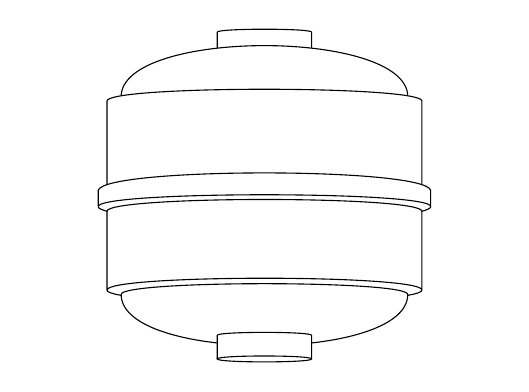
\begin{tikzpicture}
    %%%% North Endcap %%%%%%%%%%%%%%%%%%%%%%%%%%%%%%%%%%%%%%%%%%%%%%%%%%%%
    \begin{scope}[yscale=-1,fill=white]
      \draw[black,xscale=0.3,yscale=0.25,yshift=-7.1cm,fill=white]
           (-2,-1.2) coordinate (a)
        -- coordinate (ab) (-2,0) coordinate (b)   
        .. coordinate (bc) controls (-2,0.2) and (2,0.2) .. (2,0) coordinate (c)
        -- (2,-1.2) coordinate (d)
        .. coordinate (de) controls (2,-1.4) and (-2,-1.4) .. (-2,-1.2) coordinate (e);
      \draw[black,xscale=0.91,yscale=0.91,yshift=-.18cm,fill=white]
           (-2,-1.2) coordinate (sea)
        .. coordinate (ad) controls (-2,-1.0) and (2,-1.0) .. (2,-1.2)
        .. coordinate (de) controls (2,-2.15) and (-2,-2.15) .. (-2,-1.2) coordinate (-2,-1.2);
    \end{scope}

    %%%% Barrel %%%%%%%%%%%%%%%%%%%%%%%%%%%%%%%%%%%%%%%%%%%%%%%%%%%%%%%%%%
    \draw[black,fill=white]
          (-2,-1.2) coordinate (a)
       -- coordinate (ab) (-2,1.2) coordinate (b) 
       .. coordinate (bc) controls (-2,1.4) and (2,1.4) .. (2,1.2) coordinate (c)
       -- (2,-1.2) coordinate (d)
       .. coordinate (de) controls (2,-1.4) and (-2,-1.4) .. (-2,-1.2) coordinate (e)
       .. coordinate (ad) controls (-2,-1.0) and (2,-1.0) .. (d);

    \draw[black,fill=white]
         (-2.11,-.13)
      -- ++(0,.2)
      .. controls (-2,.36) and (2,.36) .. (2.11,.07)
      -- ++(0,-.2);

    \draw[black,fill=white]
         (-2,-.2)
      .. controls (-2,0) and (2,0) .. ( 2,-.2)
      .. controls (3,.08) and (-3,.08) .. (-2,-.2) --cycle;

    %%%% South Endcap %%%%%%%%%%%%%%%%%%%%%%%%%%%%%%%%%%%%%%%%%%%%%%%%%%%%
    \begin{scope}
    \draw[xscale=0.91,yscale=0.91,yshift=-.18cm,fill=white]
         (-2,-1.2) coordinate (sea)
      .. coordinate (ad) controls (-2,-1.0) and (2,-1.0) .. (2,-1.2)
      .. coordinate (de) controls (2,-2.15) and (-2,-2.15) .. (-2,-1.2) coordinate (-2,-1.2);
    \draw[xscale=0.3,yscale=0.25,yshift=-7.1cm,fill=white]
         (-2,-1.2) coordinate (a)
      -- coordinate (ab) (-2,0) coordinate (b) 
      .. coordinate (bc) controls (-2,0.2) and (2,0.2) .. (2,0) coordinate (c)
      -- (2,-1.2) coordinate (d)
      .. coordinate (de) controls (2,-1.4) and (-2,-1.4) .. (-2,-1.2) coordinate (e)
      .. coordinate (ad) controls (-2,-1.0) and (2,-1.0) .. (d);
    \end{scope}
\end{tikzpicture}
